%\documentclass[12pt, preprint,numberedappendix]{emulateapj}
%\documentclass[12pt, preprint]{aastex}
%\documentclass[apj]{emulateapj}
\documentclass[12pt, letterpaper]{article}

%\newcommand\submitms{n}		% set to y to follow AAS ``ms'' names, etc.
%\newcommand\bibinc{n}		% set to y if bib pasted in .tex, set to n to use bibtex


%\usepackage{pdfsync}
%\usepackage{subeqnarray}
\usepackage[top=1in, bottom=0.8in, left=1in, right=1in]{geometry}
\usepackage{natbib}
\usepackage{color}
\usepackage{graphicx}
\usepackage{fancyhdr}
\usepackage[T1]{fontenc}
\usepackage{titling}
\usepackage{sectsty}
\usepackage{sidecap}
\usepackage{placeins}
\usepackage{indentfirst}
\usepackage{wrapfig}
\setlength{\droptitle}{-7em}
\setlength{\abovecaptionskip}{-0.4ex}
\setlength{\belowcaptionskip}{-0.4ex}
%\pagenumbering{gobble}
\pagestyle{fancy}
\lhead{Ana-Maria Piso}
\rhead{Sagan Fellowship Current and Previous Research Statement}
\date{}
%\rhead{\thepage}


%\bibliographystyle{apj}

\title{Sagan Fellowship Previous and Current Research Statement: \\
Giant Planet Formation and Snowlines in Protoplanetary Disks}
\author{Ana-Maria Piso}

%\newenvironment{packed_item}{
%\begin{itemize}
%  \setlength{\itemsep}{1pt}
%  \setlength{\parskip}{0pt}
%  \setlength{\parsep}{0pt}
%}{\end{itemize}}

\begin{document}
\maketitle

%\slugcomment{Draft Modified \today}

\vspace{-0.8cm}


Planets are born in protoplanetary disks, which means that their structure and composition are determined by and highly connected to the chemical composition and structure of the disk in which they form. In my current and previous research, I have approached this intricate disk-planet link from two directions: (1) by exploring the core accretion mechanism, specifically calculating the minimum required core mass to form a gas giant before the dissipation of the gas in the protoplanetary disk, and (2) by understanding how disk chemistry and dynamics shape the snowline locations of volatiles in disks, which has direct implications for the chemical composition of extrasolar planet (exoplanet) atmospheres. 

\vspace{0.2in}

%\section{Coupled Chemical and Dynamical Disk Evolution} 
\underline{\textbf{Minimum Core Masses for Giant Planet Formation}}

Gas giants are widely believed to form through core accretion (Stevenson 1982, Pollack et al. 1996), a theory in which solid protoplanetary cores grow large enough to accumulate a massive atmosphere. This is particularly challenging in the outer parts of a disk, where long dynamical times make it difficult for a core to grow fast enough before the gas disk dissipates on a timescale of a few million years. At the same time, however, giant planets on wide orbits have been discovered in recent years, such as the HR 8799 system (Marois et al. 2008). This poses an intriguing question: how did these planets form? In this part of my research, I attempted to address this issue ? specifically, what is the lowest possible core mass required to form a gas giant before disk dissipation? We start investigating this issue in Piso & Youdin (2014), where we develop a core accretion model complementary to most state-of-the-art planet formation models, which assume that a giant planet?s core and atmosphere grow simultaneously (Bodenheimer & Pollack 1986, Wuchterl 1993, Rafikov 2006). Specifically, we assume that planetesimal accretion is negligible, and instead the envelope accretes gas while undergoing Kelvin-Helmholtz contraction. This gives a lower limit on the minimum (critical) core mass, Mcrit, to form a giant planet, since additional planetesimal accretion in this stage would heat up the atmosphere, inhibit its ability to cool, thus increasing the critical core mass. Moreover, while Mcrit has been systematically computed as a function of disk properties and stellocentric separation for steady-state atmospheres heated by planetesimal accretion (Rafikov 2006), no equivalent systematic study is available for this minimum value of Mcrit. We develop such a study by considering envelopes accreting around fully formed cores at distances between 5 and 100 astronomical units (AU) from their host star. We use a simple model that assumes the nebular gas to be ideal and polytropic, and that the dust opacity is the standard interstellar opacity (ISM; Bell & Lin 94). We find Mcrit to decrease between 8.5 Earth Masses (ME) at 5 AU to 3.5 ME at 100 AU. These results are lower than those of standard studies, which typically assume Mcrit ~ 10 ME (Stevenson 1982). Our study hence makes great strides in understanding the formation of giant planets at large separations. Moreover, our numerical technique has been used by Lee et al. (2014) and Lee et al. (2015) to understand planet formation in the inner disk. 

\begin{wrapfigure}{r}{0.5\textwidth}
  \begin{center}
    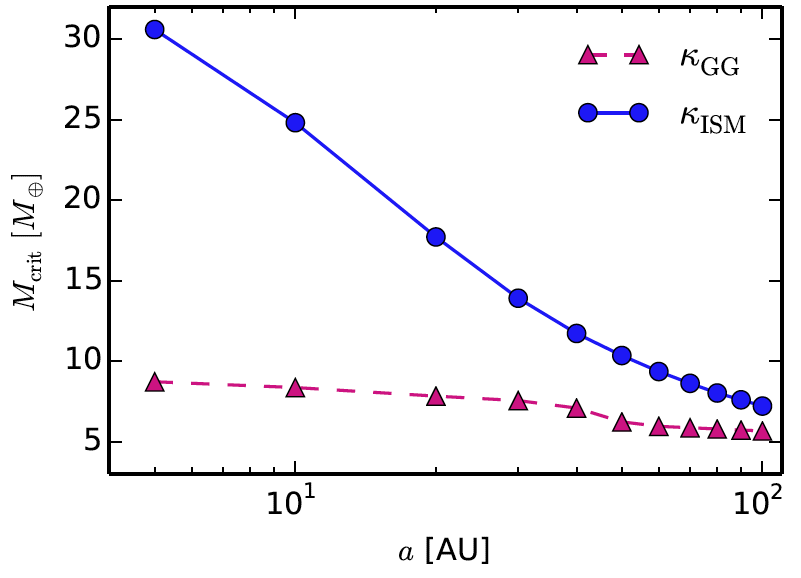
\includegraphics[width=0.5\textwidth]{Mcrit_vs_a_gg}
  \end{center}
  \caption{A gull}
\end{wrapfigure}

The idealized model developed in Piso & Youdin (2014) neglects realistic effects, such as the fact that the nebular gas is non-ideal (Saumon et al. 1995), as well as that the dust opacity is likely to be lower than the ISM one due to grain growth (Pollack 1985). In Piso, Youdin & Murray-Clay (2015), we improve our model by including these effects. We use the Saumon et al. (1995) EOS tables, and we extend them to lower temperatures and pressures as suitable for the parameter space we are exploring. These tables are available upon request and may prove useful to understand planet formation in the outer disk. Moreover, we use realistic opacity tables that take into account grain growth (D?Alessio et al. 2001) to calculate Mcrit. We find that a realistic EOS increases Mcrit, while grain growth opacities, in contrast, decrease Mcrit. Taking these two competing effects together, we calculate Mcrit ~ 8 ME at 5 AU, decreasing to 5 ME at 100 AU. Our results are still lower than 10 ME, the typically quoted value, and may be up to one order of magnitude lower if grain coagulation is taken into account (see Piso, Youdin & Murray-Clay 2015 for details). Our work provides further insight into giant planet formation, and is a rich field of research to pursue. 


\vspace{0.2in}
%\section{Planet and Planetesimal Migration}
\underline{\textbf{Snowline Locations in Protoplanetary Disks}}

A. H2O, CO2, CO Snowlines and the C/O ratio	
The locations of volatile snowlines in protoplanetary disks are a defining feature of both gas giant and protoplanetary disk chemistry, as they provide vital information about the abundance of these molecules in gas and dust throughout the disk. In this part of my dissertation and beyond, I want to understand the disk well enough to (1) predict what kind of planet compositions result from planet formation in different parts of the disk, and (2) back-track the planet formation location based on planet composition. While disk structure is very complex, we do have valuable observational evidence of molecular abundance detections in disks (Henning & Semenov 2013), as well as volatile snowlines (Qi et al. 2013, Zhang et al. 2013). One important signature of disk and exoplanet chemistry is the carbon-to-oxygen (C/O) ratio. Specifically, an important consequence of snowline formation in disks is that disks are expected to present different C/O ratios in the gas and in icy dust mantles at different disk radii. This effect was quantified by �berg et al. (2011), who considered the fact that the main carries of carbon and oxygen, i.e. H2O, CO2 and CO, have different condensation temperatures. This changes the relative abundance of C and O in gaseous and solid form as a function of the snowline location of the volatiles mentioned above. In Piso, �berg, et al. (2015), we improve on this model by including the effect of radial drift of solids and viscous gas accretion on the volatile snowline locations. We use a simple, semi-analytical model to solve for the coupled drift-desorbed equations for particles of different initial sizes, as well as for various disk models (irradiated, evolving, viscous). For all disks, we find that particles within an initial size range desorb at a size-dependent location in the disk, which is independent of the particle's initial position. From this, we can estimate upper limits for the C/O ratio in disks (see Piso, �berg, et al. 2015 for details). The largest desorbing particles in our model have initial sizes of ~7 m, and they are representative for the snowline locations, as realistic grain size distributions are dominated in mass by the largest particles. We thus obtain a very powerful result: radial drift and gas accretion may move the H2O, CO2 and CO snowlines by up to 40-60\% compared to a static disk, which is a huge difference. For a transition disk, i.e. a disk with an inner cavity significantly depleted of gas, we find that H2O particles that start at an initial distance interior to the gap drift towards the original snowline, while grains located exterior to the gap stop shortly after crossing the gap edge, due to the decrease in gas pressure inside the cavity. This is qualitatively consistent with the observations of Zhang et al. (2013), which show that the H2O snowline is pushed outwards in a transition disk compared to a full disk. Our model framework is thus generally valid for more complicated disk structures as well. We plan to further improve this model by adding several disk processes, such as turbulent diffusion, particle composition and grain morphology.

\begin{wrapfigure}{l}{0.5\textwidth}
  \begin{center}
    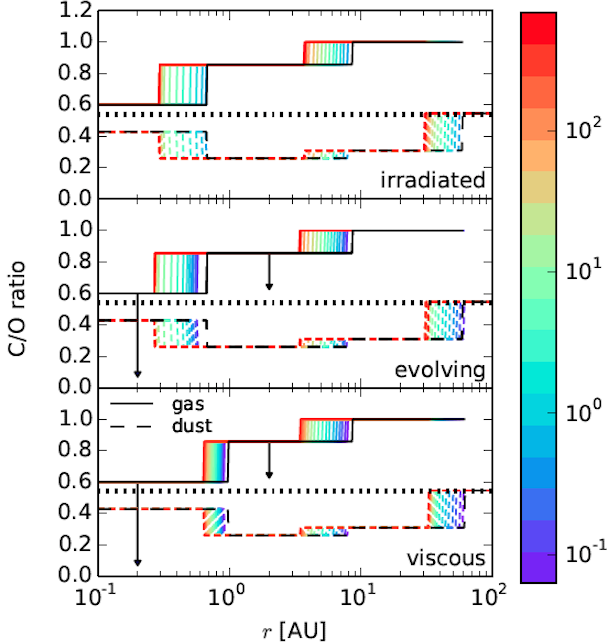
\includegraphics[width=0.5\textwidth]{C_O_ratio_passive_active_disk_many_colorbar_complete_new2}
  \end{center}
  \caption{A gull}
\end{wrapfigure}

B. Nitrogen Abundance and Ice Binding Energies
Aside from the main C and O carriers, nitrogen is an important molecule to study, as it is highly abundant in the Solar system (Lodders 2009) and disks, and primarily found as N2. In Piso et al. (in prep), we show that the nitrogen to oxygen (N/O) ratio in gas is significantly larger than the Solar abundance. This implies that the N/O ratio may be used as an additional signature of disk and exoplanet atmospheric chemistry, aside from the C/O ratio, which may give us another clue into the chemical composition of protoplanetary disks and, implicitly, of planets. Moreover, we use new results from Fayolle et al. (in prep) for the binding energies of CO and N2, mixed with H2O or as pure ices. We find that the binding energies of water-ice mixtures are significantly larger than the pure ice ones, and move the CO and N2 snowlines by at least a few AU. 


%\begin{figure}[h!]
%\centering
%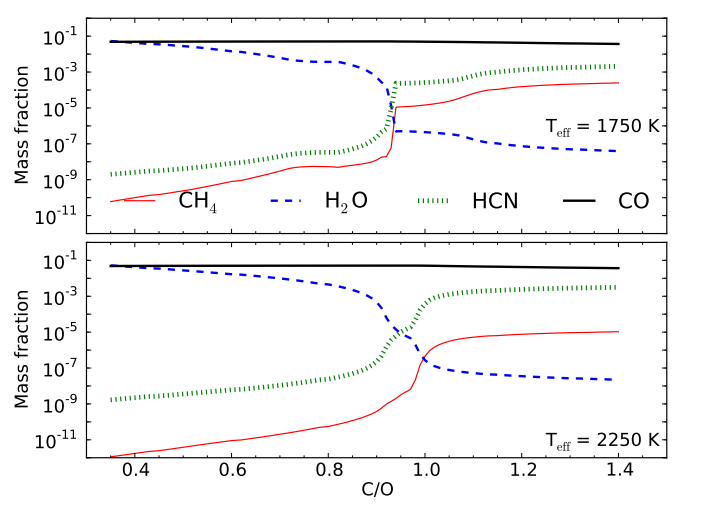
\includegraphics[width=0.7\textwidth]{CO_abundances}
%%\vspace{-0.5in}
%\caption{TBD}
%\label{fig:CO}
%\end{figure}


%\if\bibinc n
%\bibliography{refs}
%\fi
\FloatBarrier
%\def\bibfont{\footnotesize}
%\setlength{\bibsep}{0.0pt}

\section*{References}
\footnotesize
%\begin{thebibliography} {9}
\noindent $[1]$ ALMA Partnership et al., 2015, ApJ, 808, L3 \\
$[2]$ Batalha, N. M. 2014, Proceedings of the National Academy of Science, 111, 12647 \\
$[3]$ Debes, J. H., Jang-Condell, H., Weinberger, A. J., Roberge, A., \& Schneider, G. 2013, ApJ, 771, 45 \\
$[4]$ Ida, S., Lin, D. N. C., \& Nagasawa, M. 2013, ApJ, 775, 42 \\
$[5]$ Kreidberg, L., Line, M. R., Bean, J. L., et al. 2015, ArXiv e-prints, arXiv:1504.05586 \\
$[6]$ Lissauer J. J., Dawson R. I., Tremaine S., 2014, Nature, 513, 336 \\
$[7]$ \"Oberg, K. I., Murray-Clay, R., \& Bergin, E. A. 2011, ApJ, 743, L16 \\
$[8]$ Piso, A.-M. A., \& Youdin, A. N. 2014, ApJ, 786, 21 \\
$[9]$ Piso, A.-M. A., Youdin, A. N., \& Murray-Clay, R. A. 2015, ApJ, 800, 82 \\
$[10]$ Piso, A.-M. A., �berg, K.I., Birnstiel, T, \& Murray-Clay, R.M., ApJ, resubmitted after referee report \\
$[11]$ Semenov, D., \& Wiebe, D. 2011, ApJS, 196, 25
%\end{thebibliography}

%\bibliographystyle{abbrv}
%\bibliography{refs}


%\if\bibinc y
%\begin{thebibliography}
%\end{thebibliography}
%\fi


\end{document}